\documentclass[main]{subfiles} 

\begin{document}

\chapter{RESULTS AND DISCUSSION}
\section{Results}
The game has been developed with user-friendliness and simple to play approach in consideration. The following screenshots from different states throughout the game illustrate the final result:
\begin{figure}[H]
    \centering
    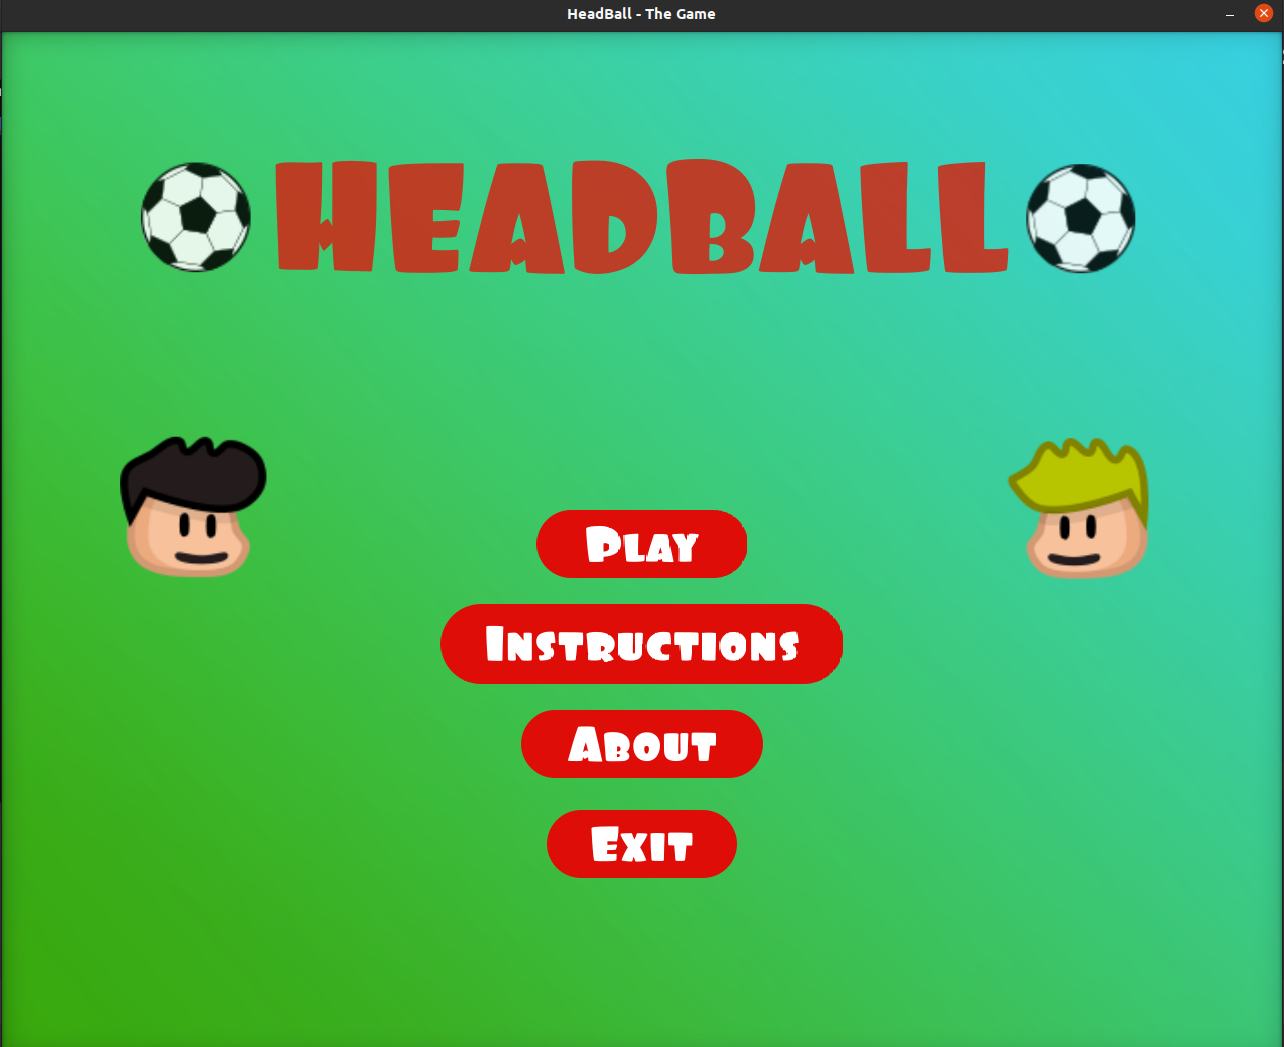
\includegraphics[scale=0.25]{graphics/state_screenshots/menu_state.png}
    \caption{Menu of the game}
    \label{fig:menu_state}
\end{figure}

\begin{figure}[H]
    \centering
    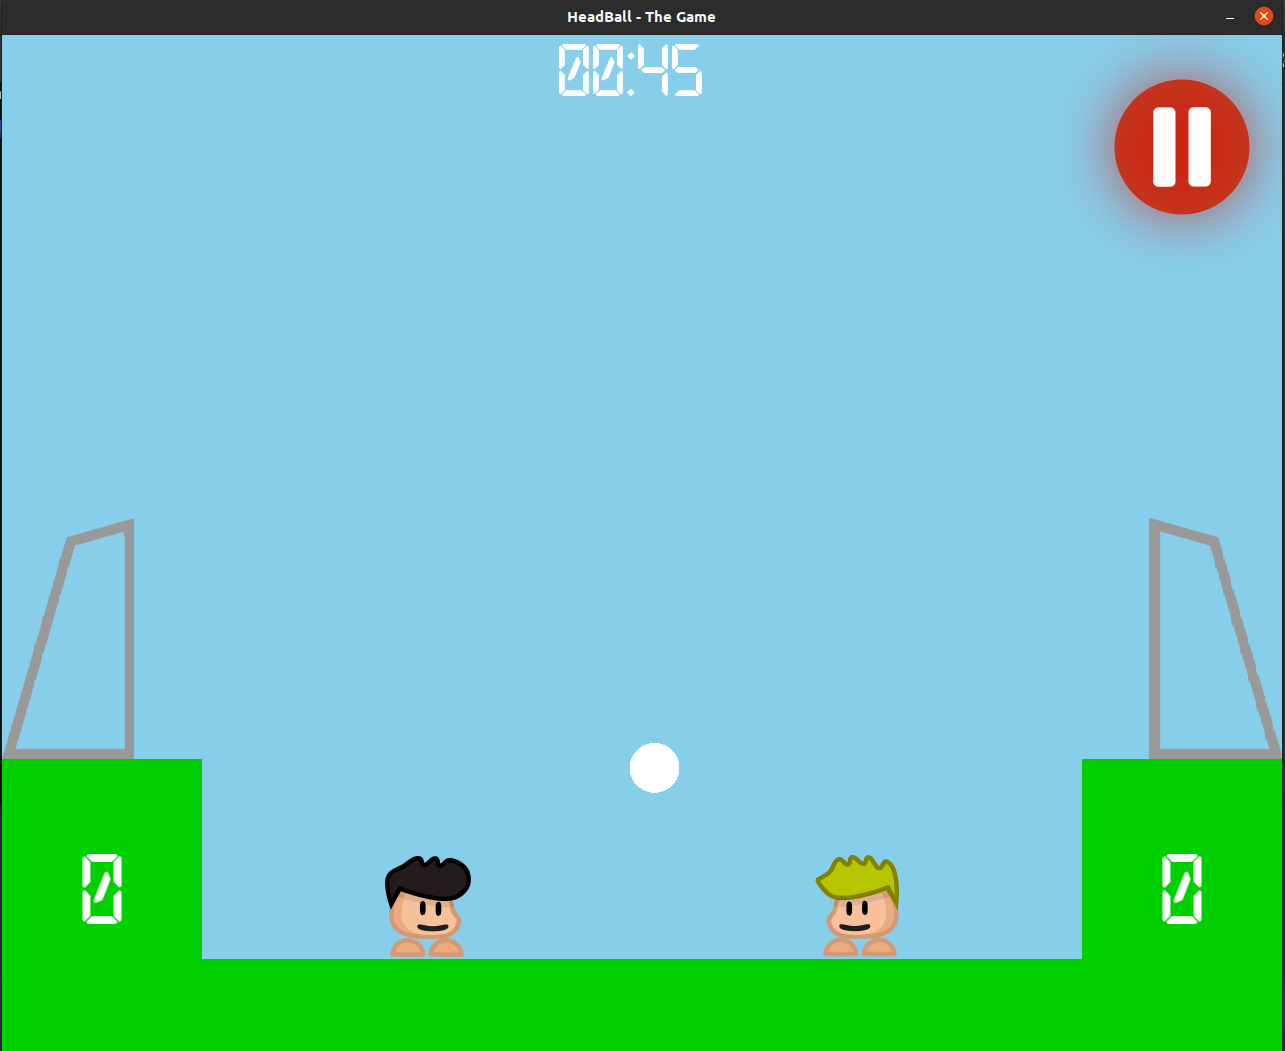
\includegraphics[scale=0.25]{graphics/state_screenshots/game_state1}
    \caption{Game Play}
    \label{fig:game_state}
\end{figure}

\begin{figure}[H]
    \centering
    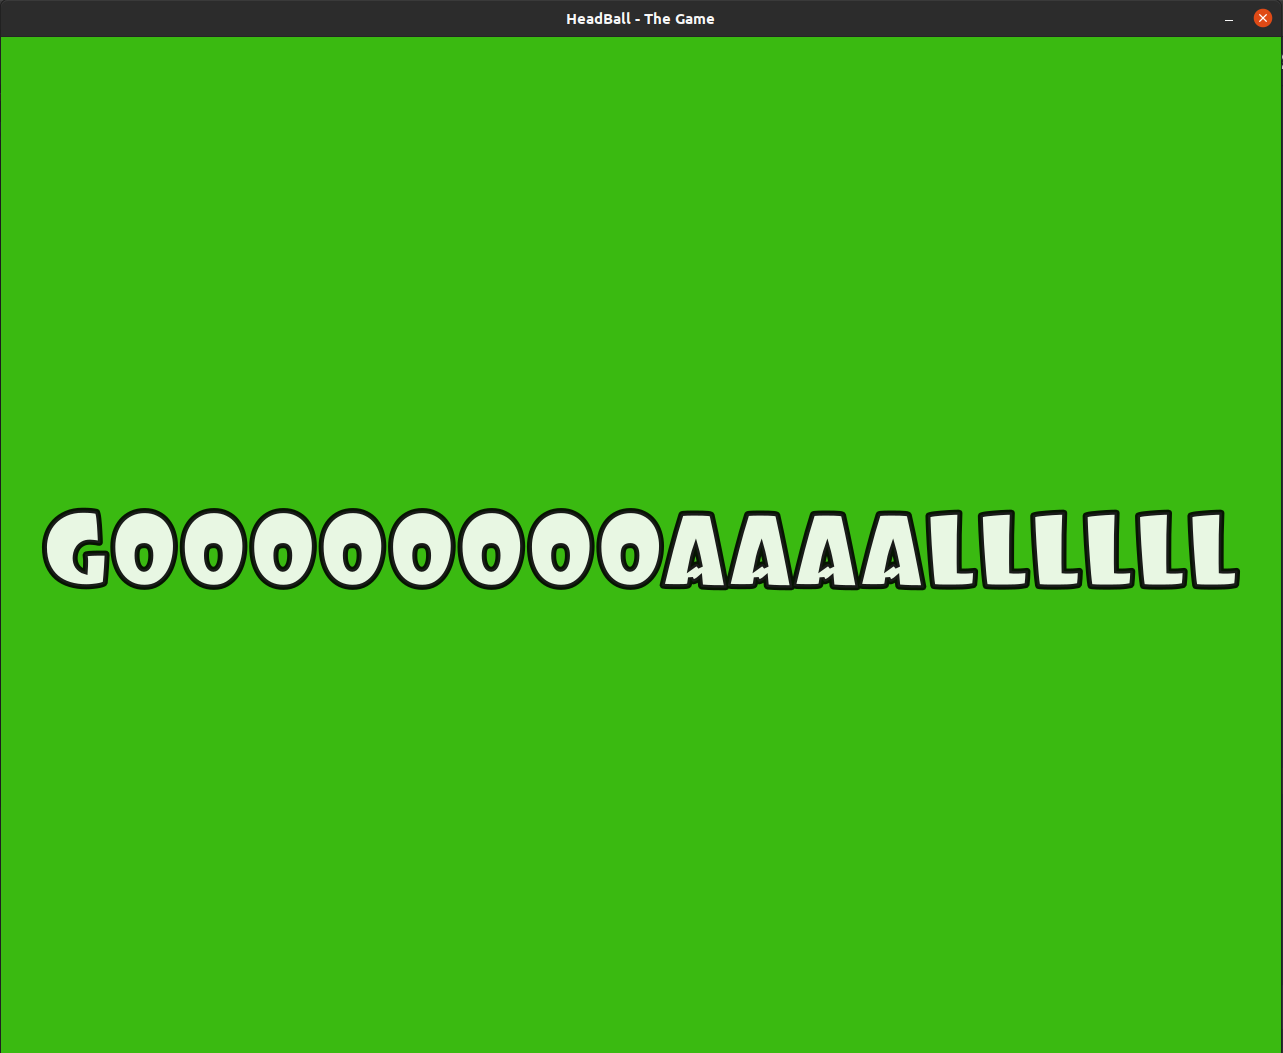
\includegraphics[scale=0.25]{graphics/state_screenshots/goal_state}
    \caption{Goal}
    \label{fig:goal_state}
\end{figure}

\begin{figure}[H]
    \centering
    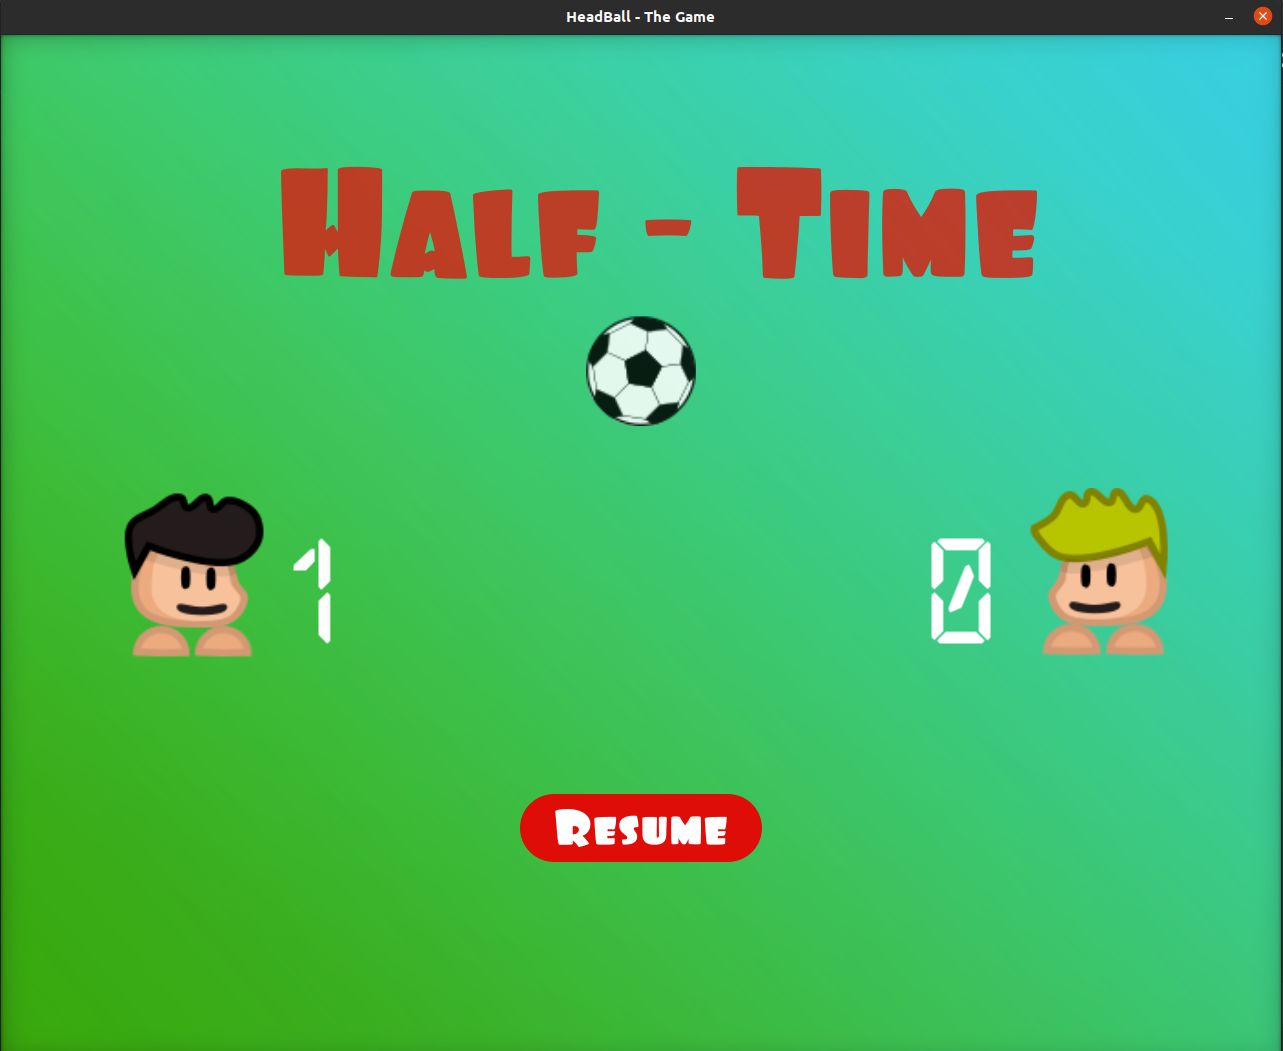
\includegraphics[scale=0.25]{graphics/state_screenshots/half_state}
    \caption{Half Time}
    \label{fig:half_state}
\end{figure}

\begin{figure}[H]
    \centering
    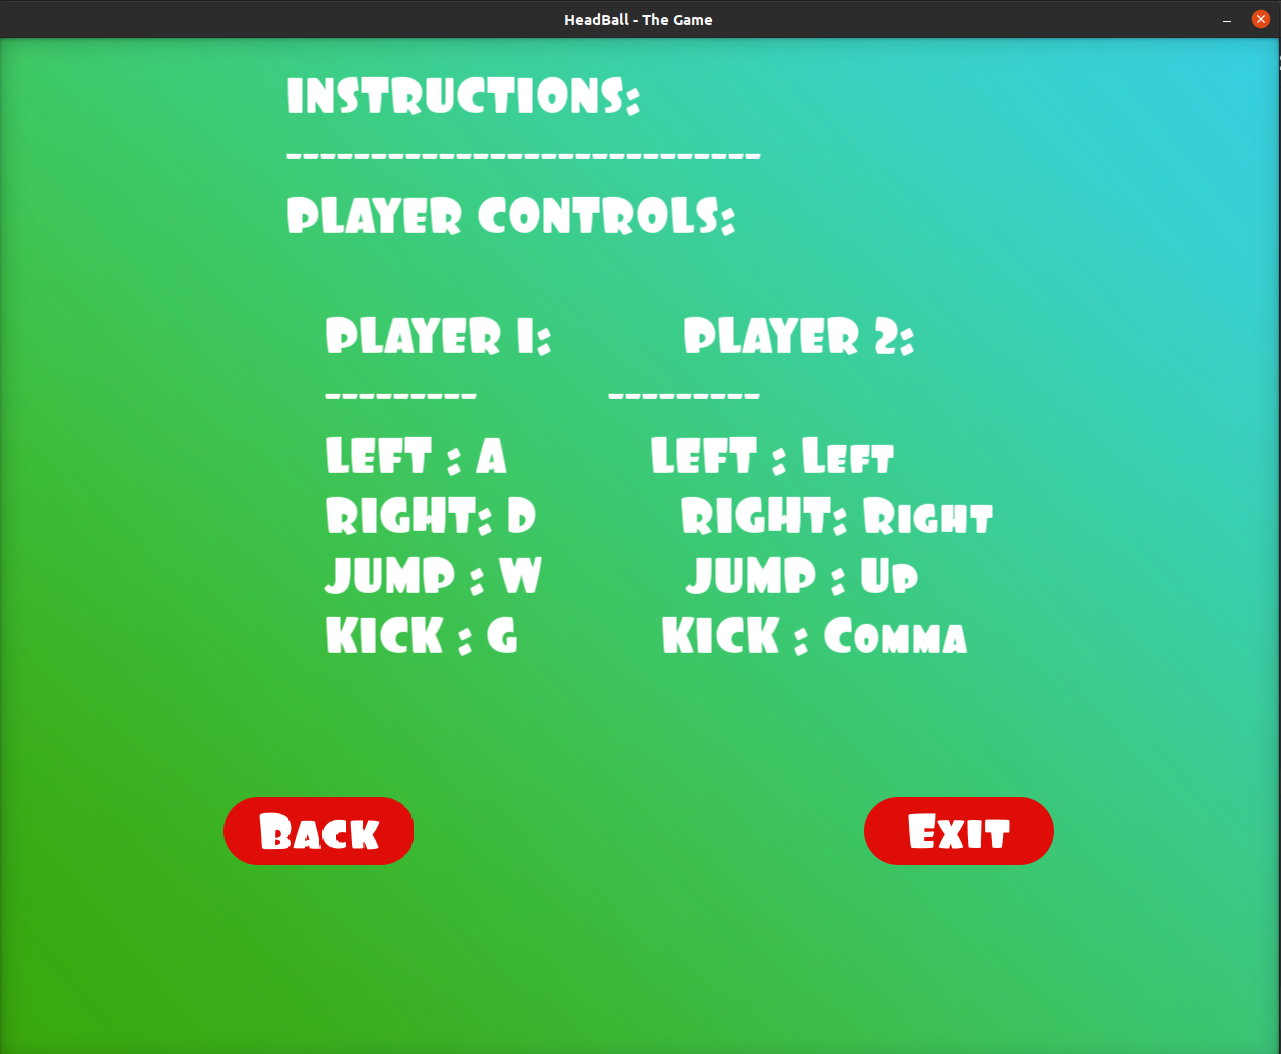
\includegraphics[scale=0.25]{graphics/state_screenshots/instructions_state}
    \caption{Instructions}
    \label{fig:instruction_state}
\end{figure}

\begin{figure}[H]
    \centering
    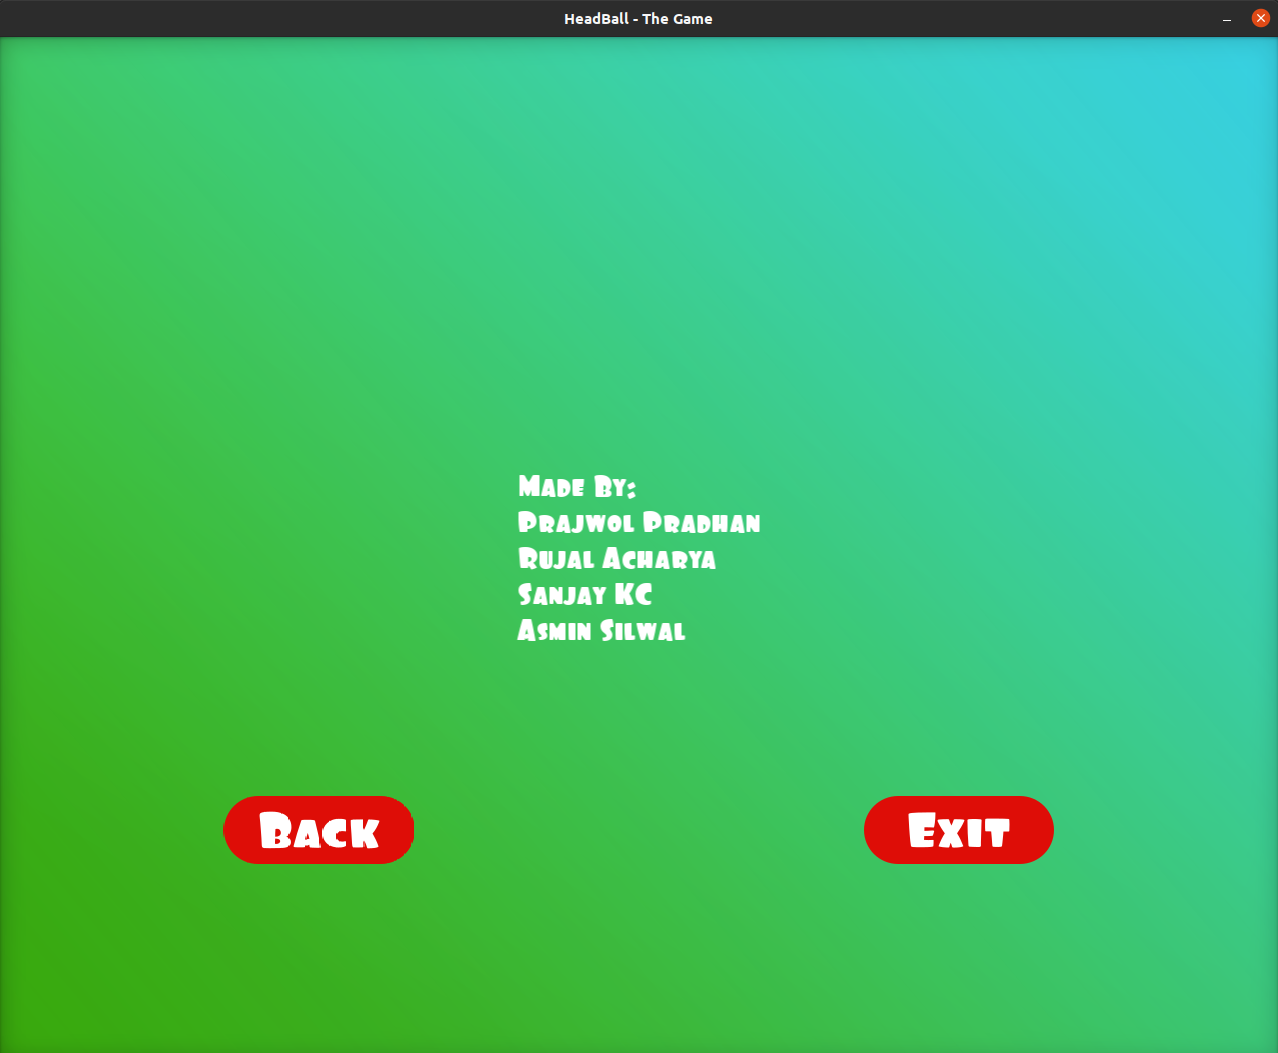
\includegraphics[scale=0.25]{graphics/state_screenshots/about_state}
    \caption{About the game}
    \label{fig:about_state}
\end{figure}

\begin{figure}[H]
    \centering
    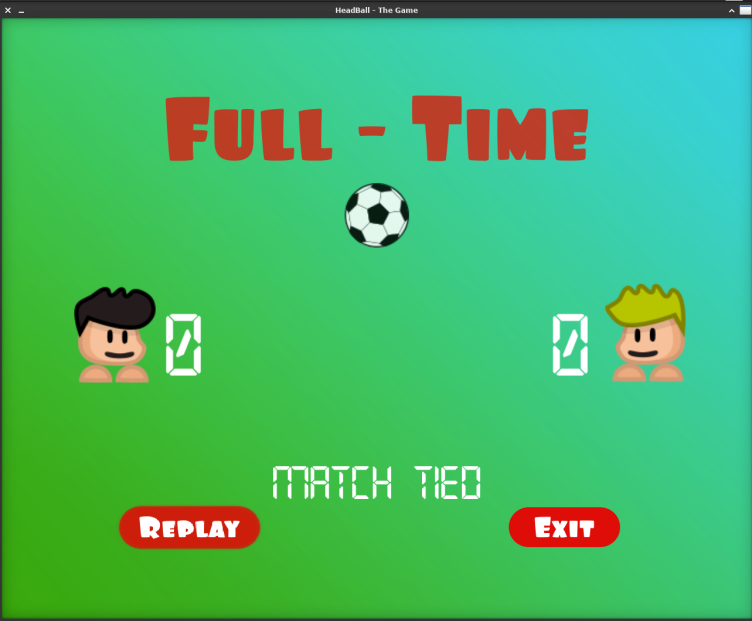
\includegraphics[scale=0.44]{graphics/state_screenshots/gameOver_state}
    \caption{Game Over}
    \label{fig:gameOver_state}
\end{figure}

\newpage

\section{Limitations}
Even though there has been put enough effort to make the game as good as possible, there still are some limitations in the game, some of those limitations are: 
\begin{enumerate}
    \item Both players should play on the same computer and use the same keyboard which probably can kill the fun of the game.
    
    \item There is no online multiplayer mode yet so the players cannot play over LAN or Internet.
    
    \item There is no Player vs Computer mode where a player can compete against the computer. 
    
    \item Currently the settings need to be configured via code only. So a common user might find it less appealing.
    
    \item The game lacks very impressive graphics.
\end{enumerate}



\section{Further Improvements}
There are many aspects of the game that can be improved. Some of them are:
\begin{enumerate}
    \item It  can  be  made  an  online  game  by adding networking capability so that two players can play from different computers over LAN or Internet.
    
    \item Voice chat and Text chat functionalities can be added in online version to make it more exciting.
 
    \item Also, Player vs Computer mode can be added so that a single player can play against the computer. 
 
    \item The graphical aspect can be further improved to make the game look more beautiful.
\end{enumerate}

\end{document}
